\tableofcontents
%%%%%%%%%%%%%%%%%%%%%%%%%%%%%%%%%%%%%
\section{Definitions}
Trough this manual we will assume that the system is installed and properly working, and that the domain where this system is installed is \verb|example.com|
To use the system, you need to open a browser compatible with html5, like Google chrome, Safari, Microsoft Internet Explorer 10+, Microsoft Edge or Mozilla Firefox, we've not tested on Opera, but it might work too.
%%%%%%%%%%%%%%%%%%%%%%%%%%%%%%%%%%%%%
\section{Login}
Proceed to the site url by opening the browser and at the address bar type: www.example.com[/install/path]\footnote{/install/path is optional and must be replaced by the installation path on the server, from the public\_html folder, relative, not absolute, so if the system is installed in ~/public\_html/checker, the url will be www.example.com/checker}
You will be presented with the following screen:

\begin{figure}[H]
	\caption{Login Screen}
	\label{img:login}
	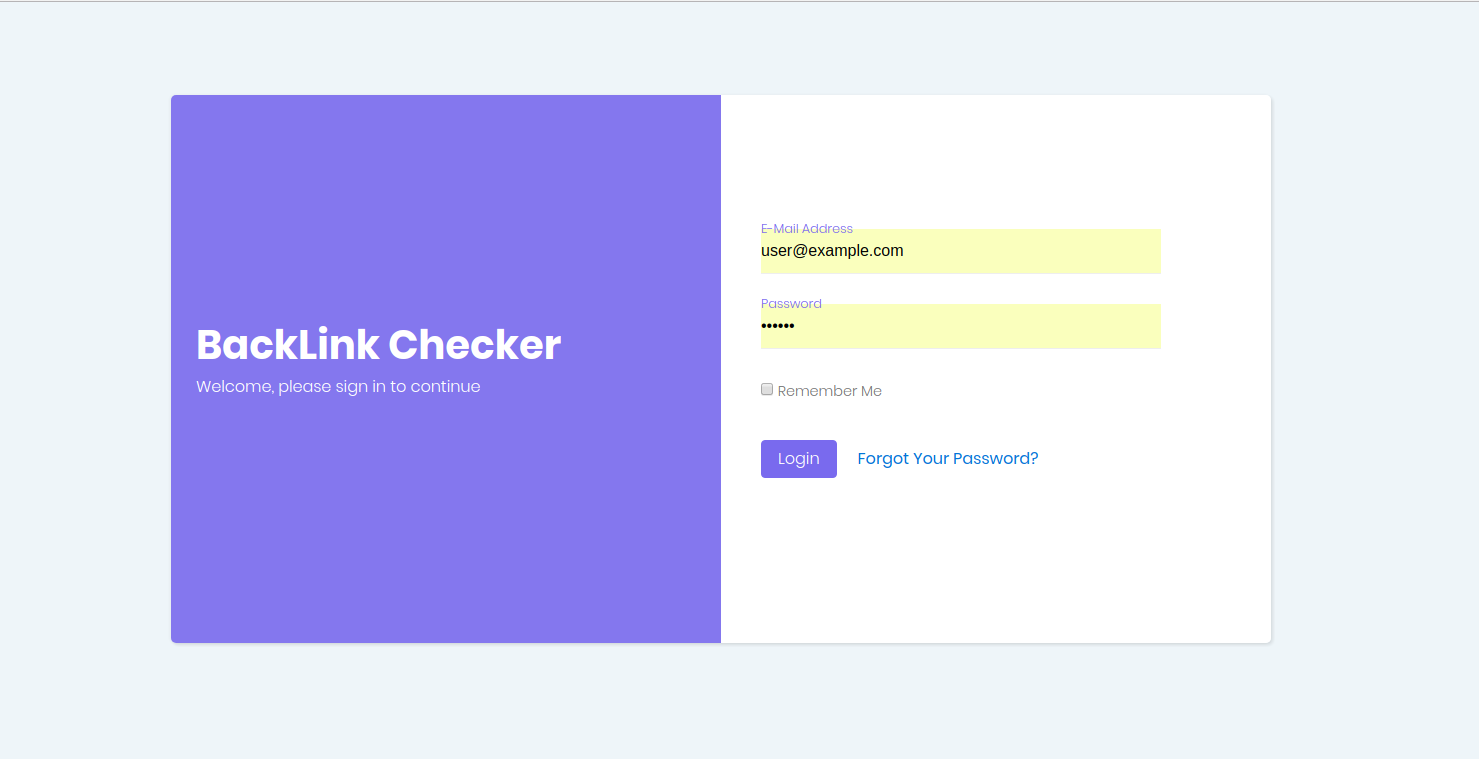
\includegraphics[width=\textwidth]{images/login_screenshot}
\end{figure}

You need to put the user name (which is the email registered), then the password and click "Login" to get into the system, if the username or password is wrong you will not be able to login.

\textbf{Note:} When the system is a fresh install with the seed option set the default admin is admin@example.com with password set to ''secretadmin'', and the low privilege user is user@example.com with password set to ''secret'' always the passwords are without quotes.

%%%%%%%%%%%%%%%%%%%%%%%%%%%%%%%%%%%%%
\section{Home}
There are two roles as designed by requirements, the admin role can do everything a user can plus add/edit/delete/block new users and manage the trash bin, the home screen for an admin will be
\begin{figure}[H]
	\caption{Admin Home Screen}
	\label{img:admin}
	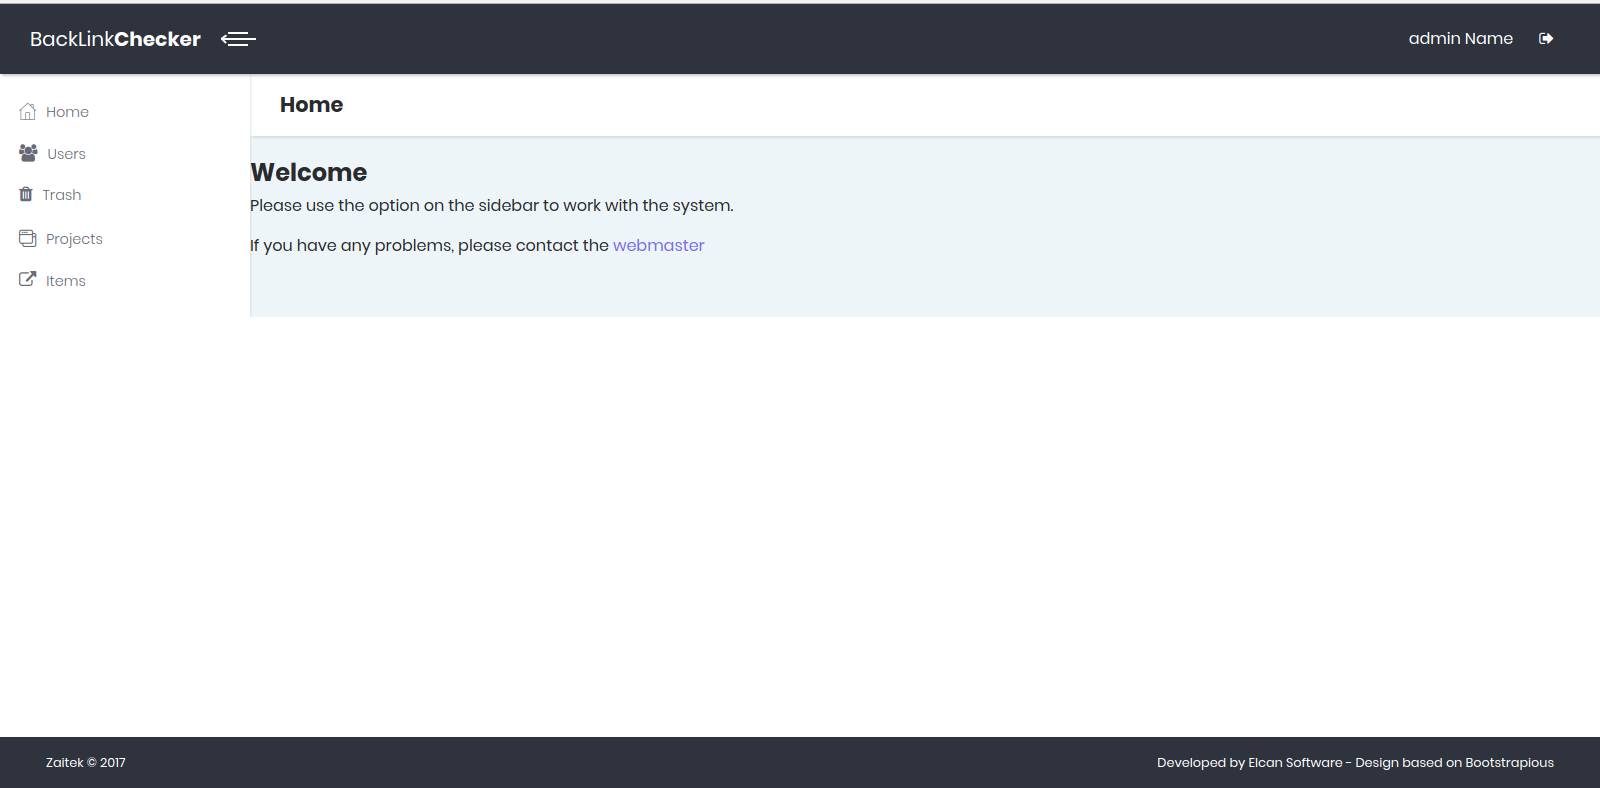
\includegraphics[width=\textwidth]{images/admin_screenshot}
\end{figure}

For a regular user, the home page will show as following:
\begin{figure}[H]
	\caption{Users Home Screen}
	\label{img:usrmng}
	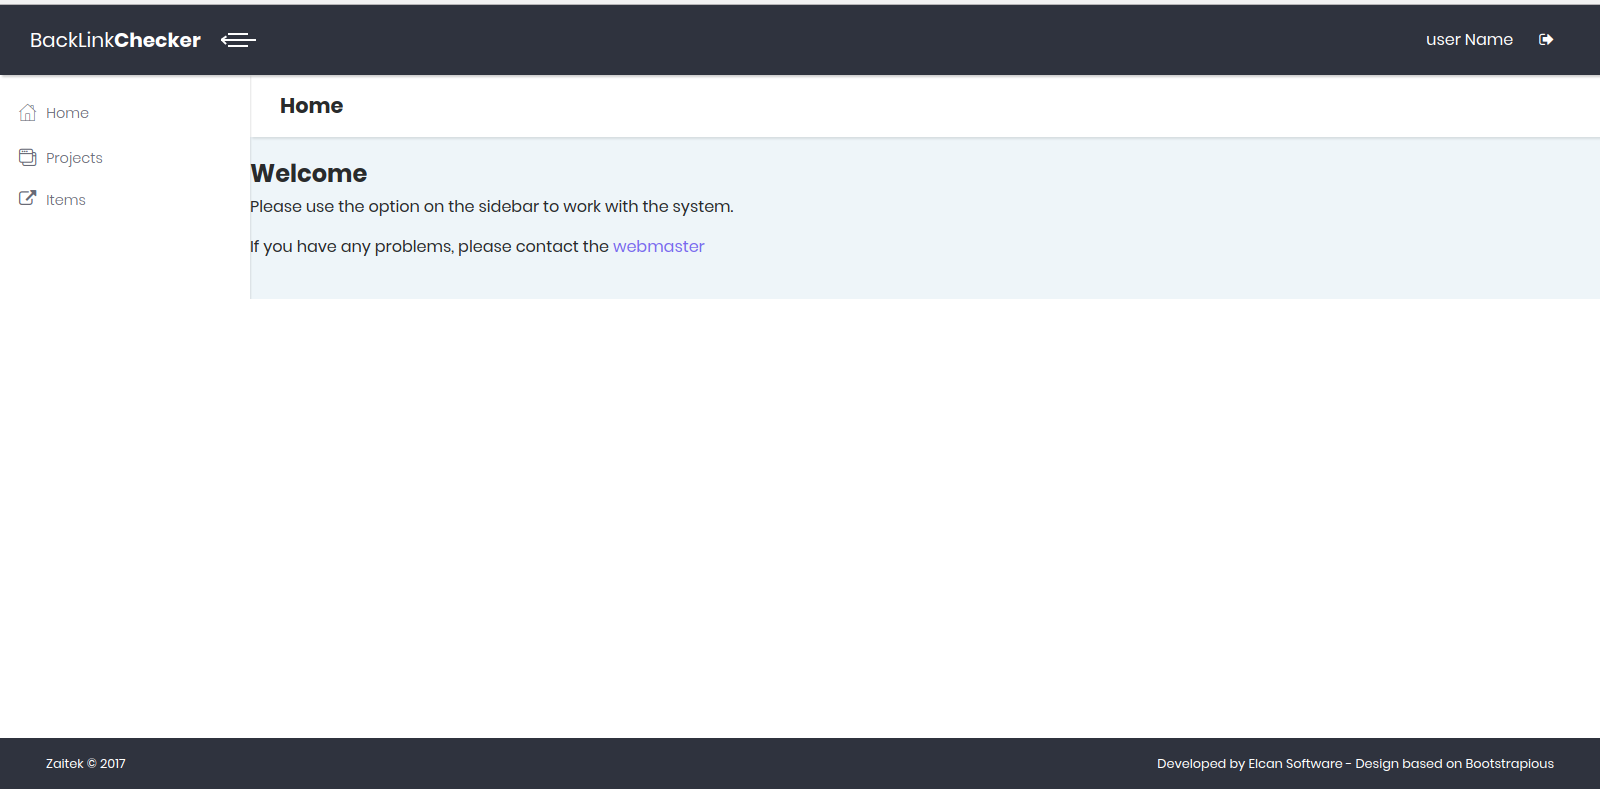
\includegraphics[width=\textwidth]{images/users_home}
\end{figure}

%%%%%%%%%%%%%%%%%%%%%%%%%%%%%%%%%%%%%
\section{As Admin}
\subsection{Users}
This section can only be accessed by the admin user, the regular user will not be able to use it. you access this section by clicking the left side bar link that states ''Users'', and you get presented a screen like the one below.
\begin{figure}[H]
	\caption{Users Main Screen}
	\label{img:usrmain}
	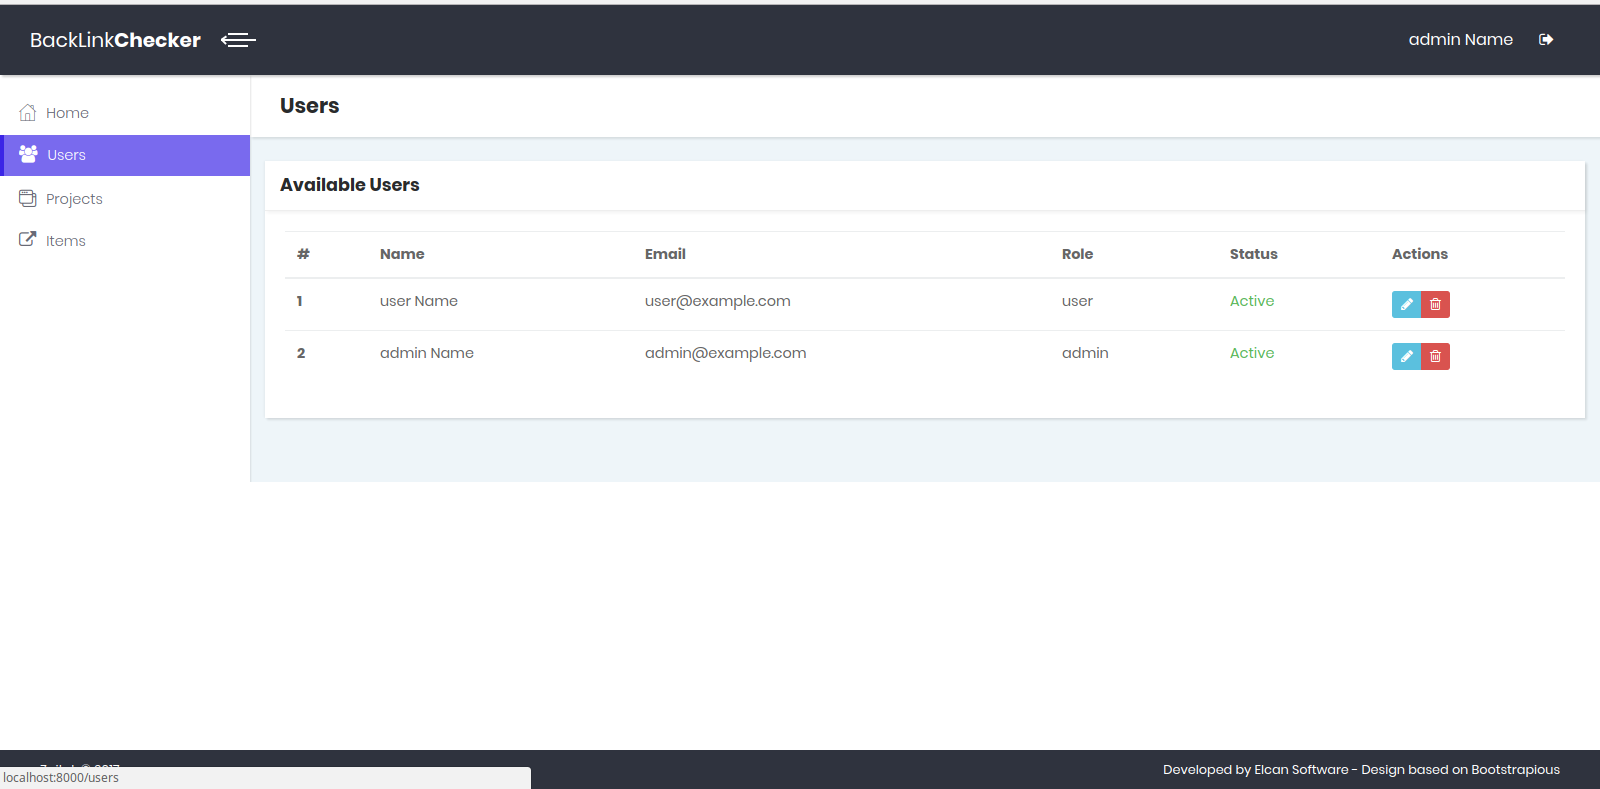
\includegraphics[width=\textwidth]{images/users_screenshot}
\end{figure}

When you click the edit link, the following form shows:
\begin{figure}[H]
	\caption{User Edit}
	\label{img:usredit}
	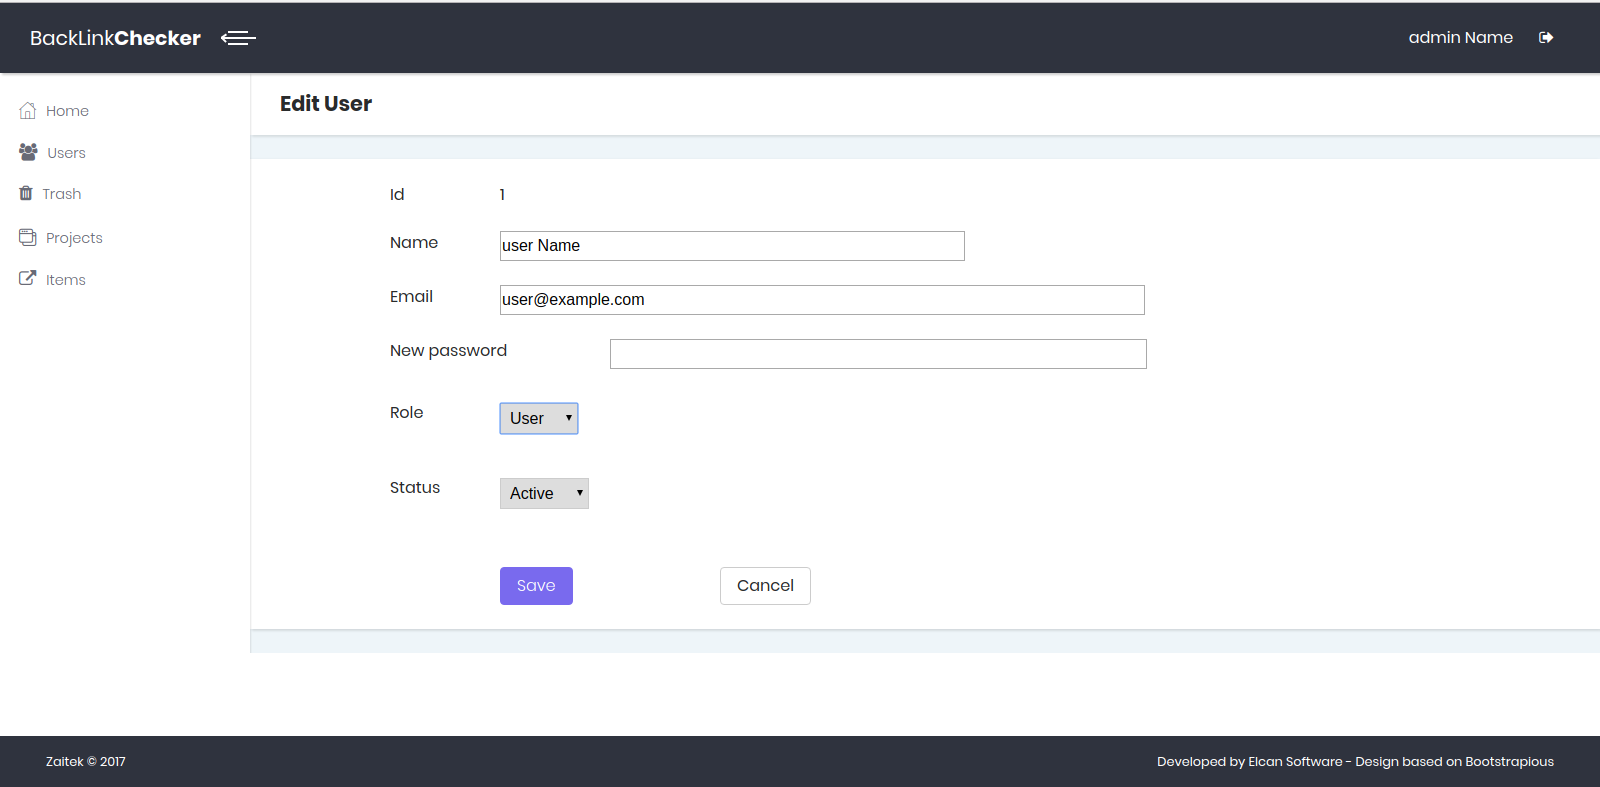
\includegraphics[width=\textwidth]{images/users_edit}
\end{figure}

After saving you get a confirmation dialog as explained in the projects section (in page \pageref{img:confirm}) with the text refering to the user.

The Add button opens the following form
\begin{figure}[H]
	\caption{User Add}
	\label{img:usradd}
	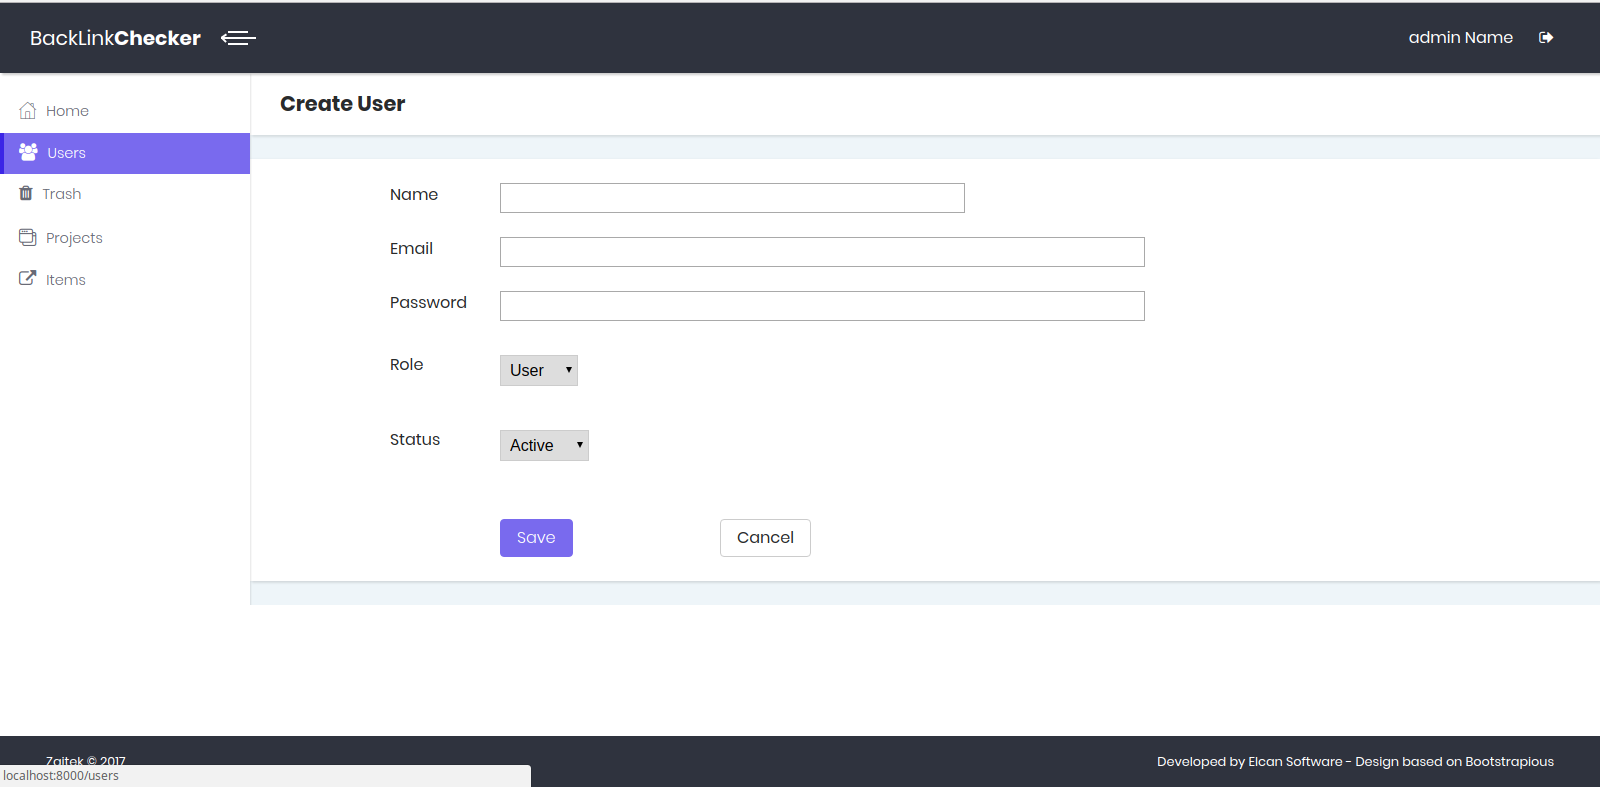
\includegraphics[width=\textwidth]{images/users_add}
\end{figure}
The Role dropdown can select any of the two available roles: Admin or User.

The 

%%%%%%%%%%%%%%%%%%%%%%%%%%%%%%%%%%%%%
\subsection{Trash}
This section is only visible to Admin users, it will list every item that has been removed by an user, and the admin will be able to remove it forever or restore, it also has an ''empty'' button to clear everything permanently. 
The interface is shown on figure \ref{img:trash}

\begin{figure}[H]
	\caption{Trash Management}
	\label{img:trash}
	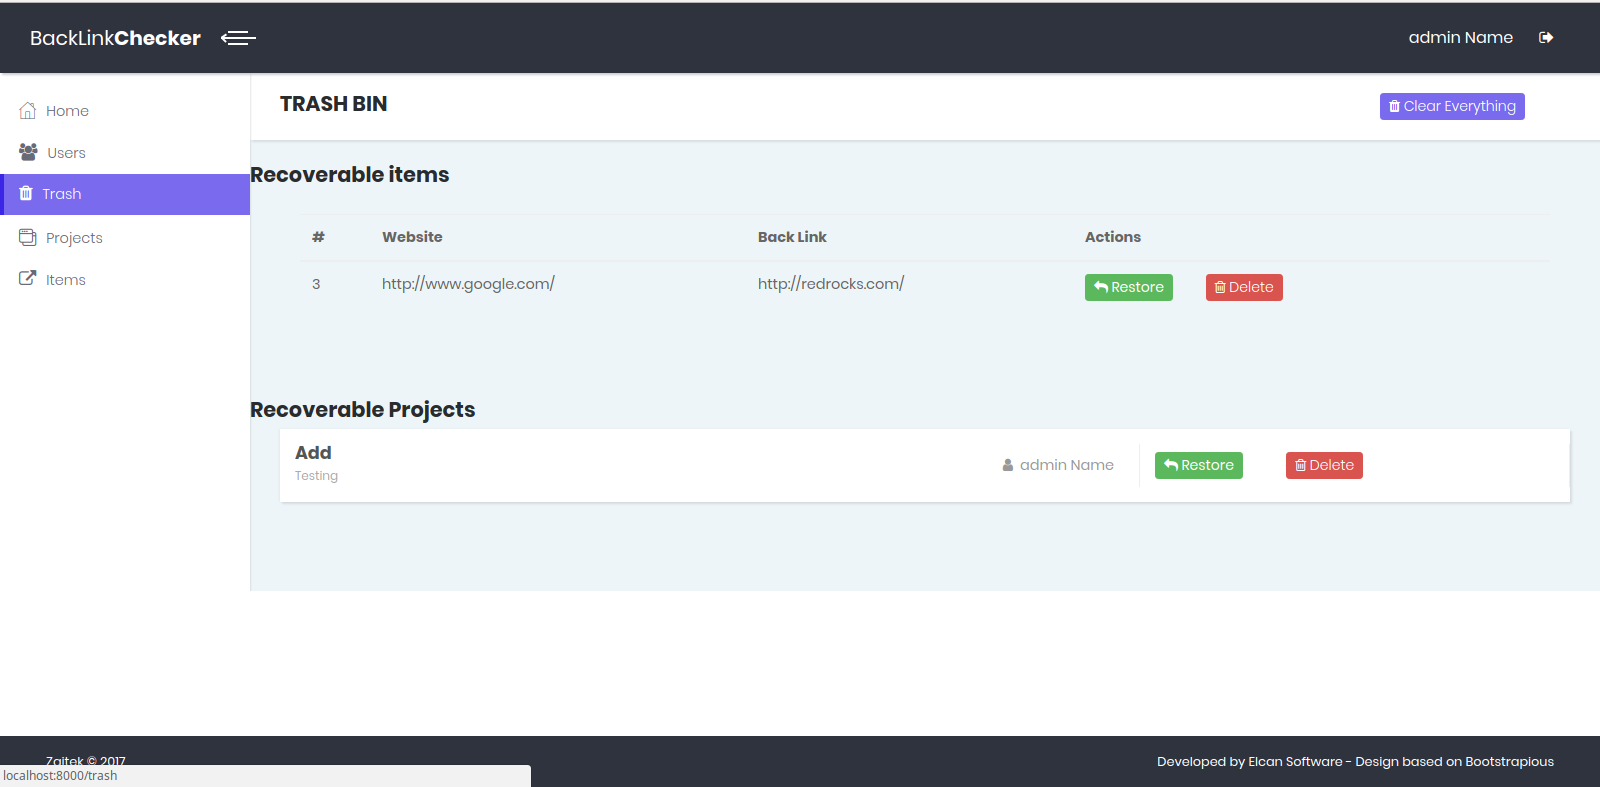
\includegraphics[width=\textwidth]{images/trash_manage.png}
\end{figure}

%%%%%%%%%%%%%%%%%%%%%%%%%%%%%%%%%%%%%
\section{Projects}
This section is accessible to all users, for the admin it will show every project in the system, for the regular user, it will only list his/her own projects.

The main screen is the one shown below:
\begin{figure}[H]
	\caption{Projects Main Screen}
	\label{img:prjmain}
	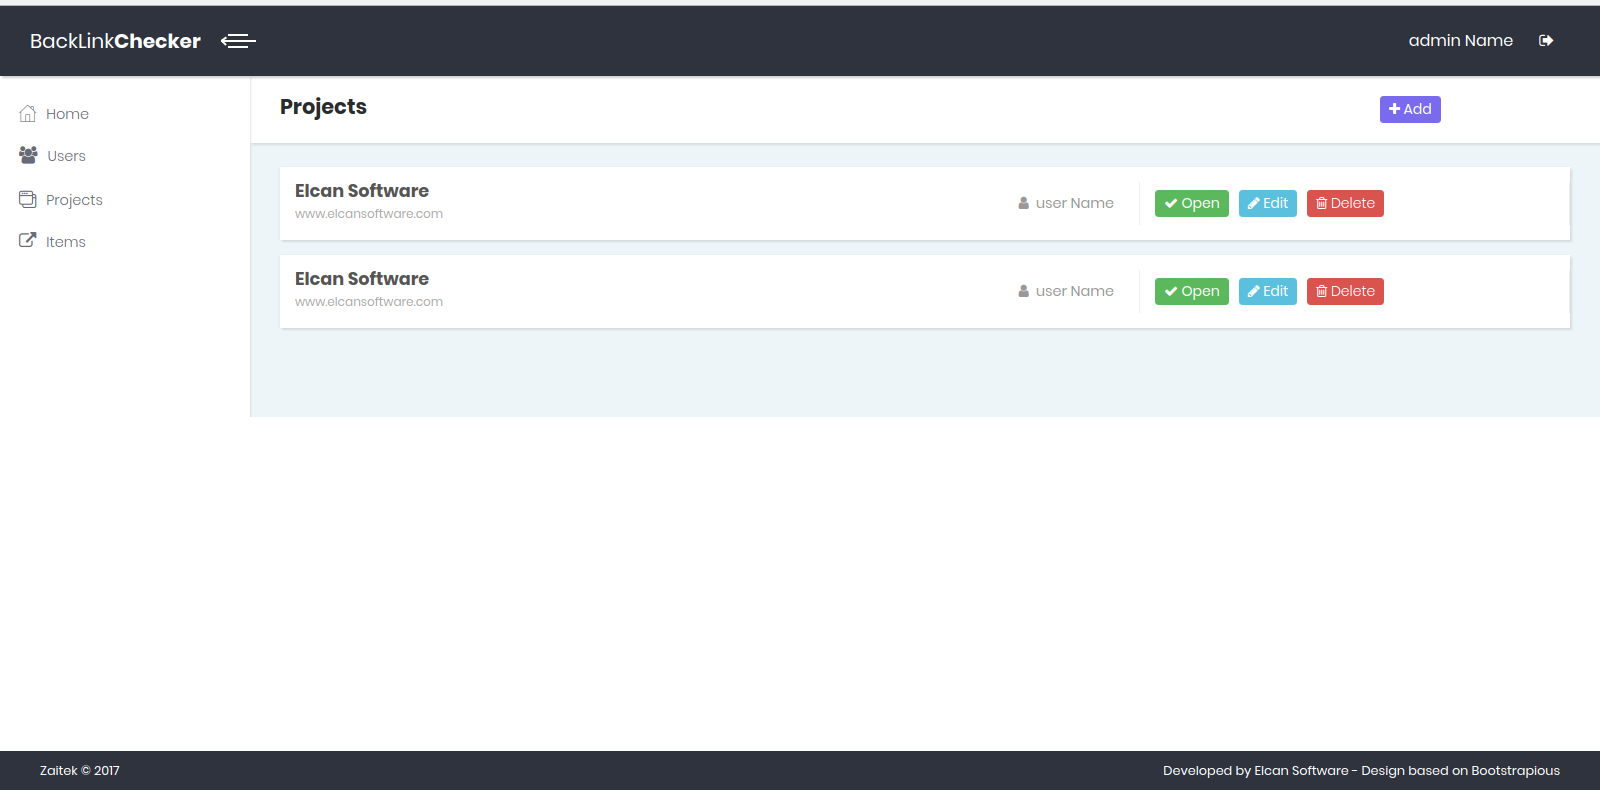
\includegraphics[width=\textwidth]{images/projects_screenshot}
\end{figure}

The +Add button opens the form to add a new project, showing the following page:
\begin{figure}[H]
	\caption{Projects Create}
	\label{img:prjcreate}
	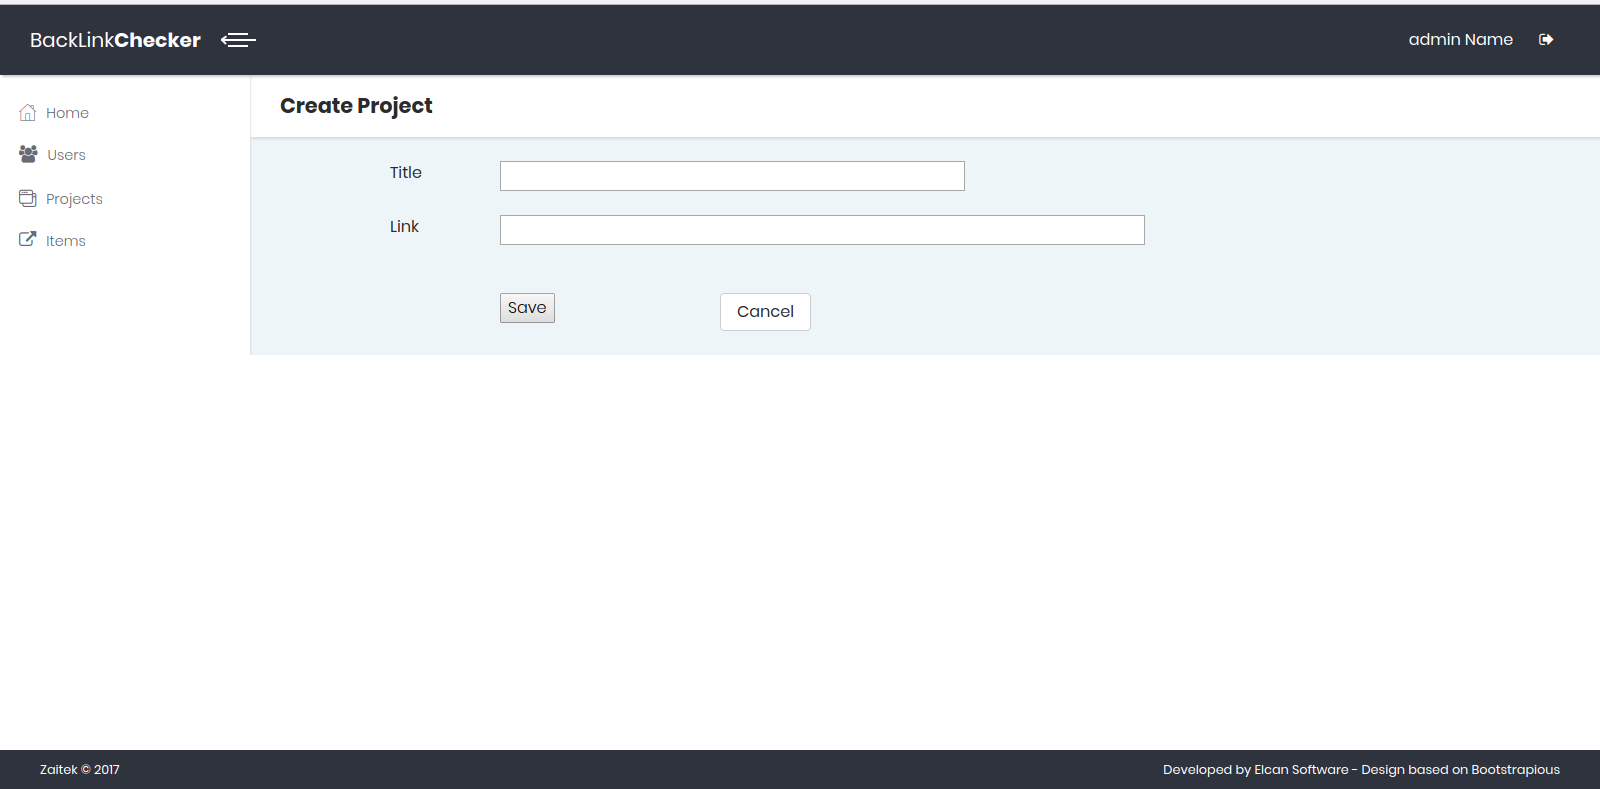
\includegraphics[width=\textwidth]{images/project_create}
\end{figure}

The same form shows if you click the EDIT button, but pre-filled with the details for the project being edited, as is shown below
\begin{figure}[H]
	\caption{Projects Edit}
	\label{img:prjedit}
	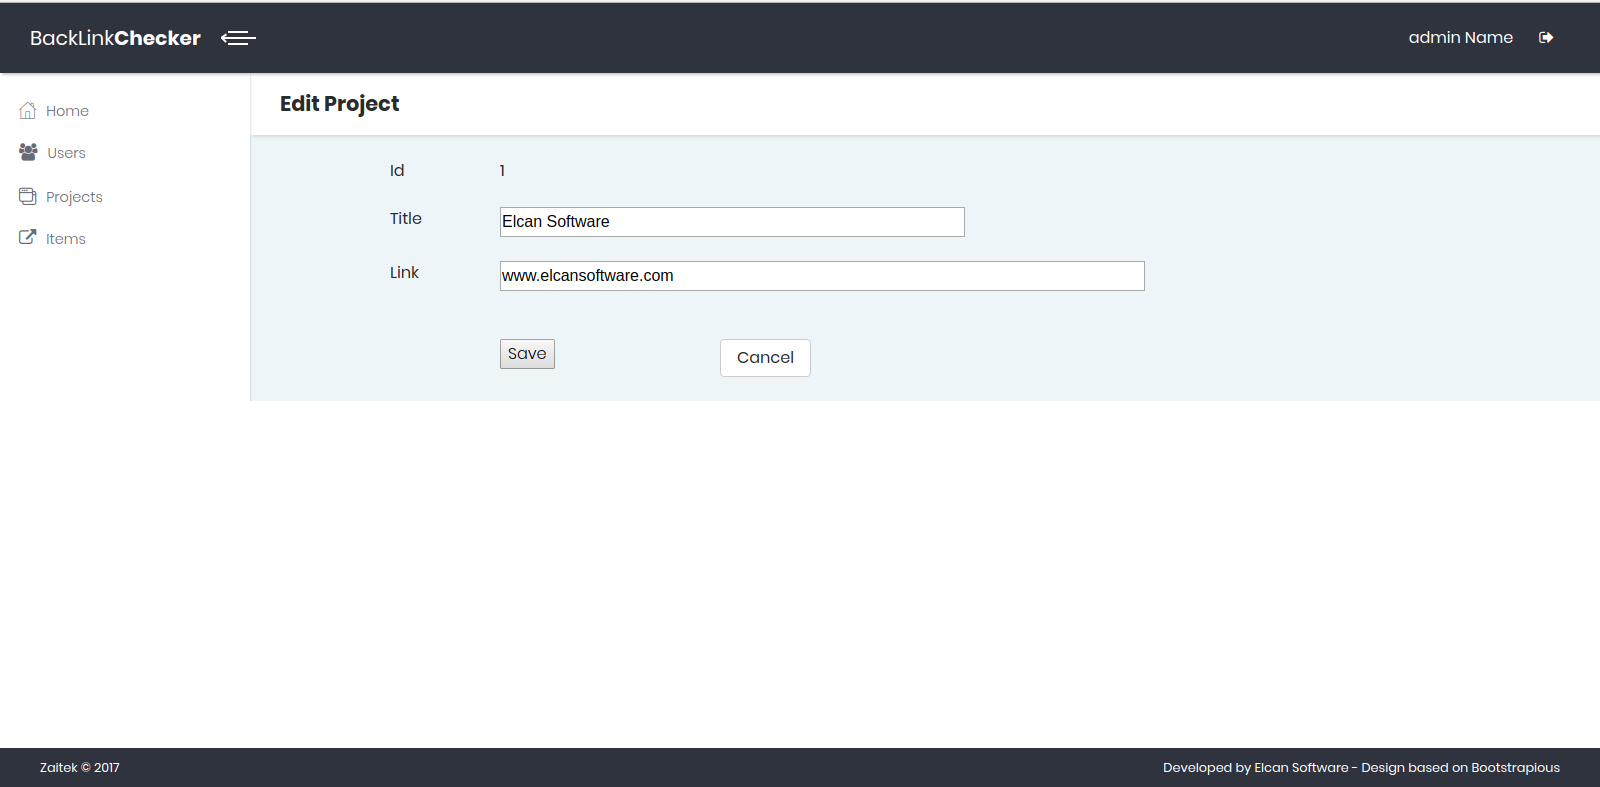
\includegraphics[width=\textwidth]{images/project_edit}
\end{figure}

After clicking save you will get a confirmation message like the one shown in figure \ref{img:confirm}
\begin{figure}[H]
	\caption{Project Save Confirmation}
	\label{img:confirm}
	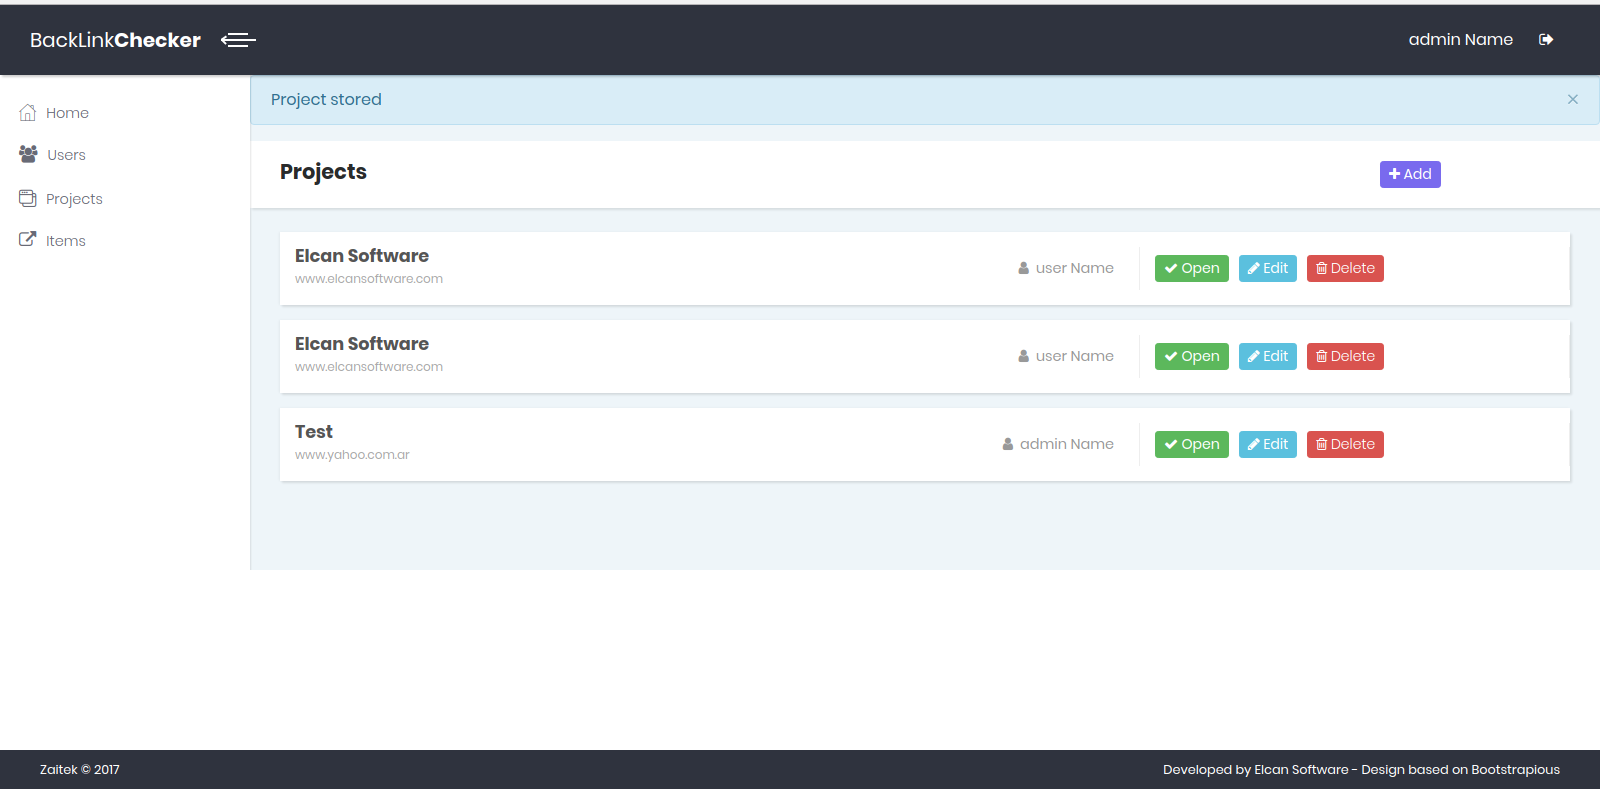
\includegraphics[width=\textwidth]{images/project_stored}
\end{figure}

The button "Open" will open the project and show the links to check, as shown on the following screen
\begin{figure}[H]
	\caption{Project Opened}
	\label{img:prjopened}
	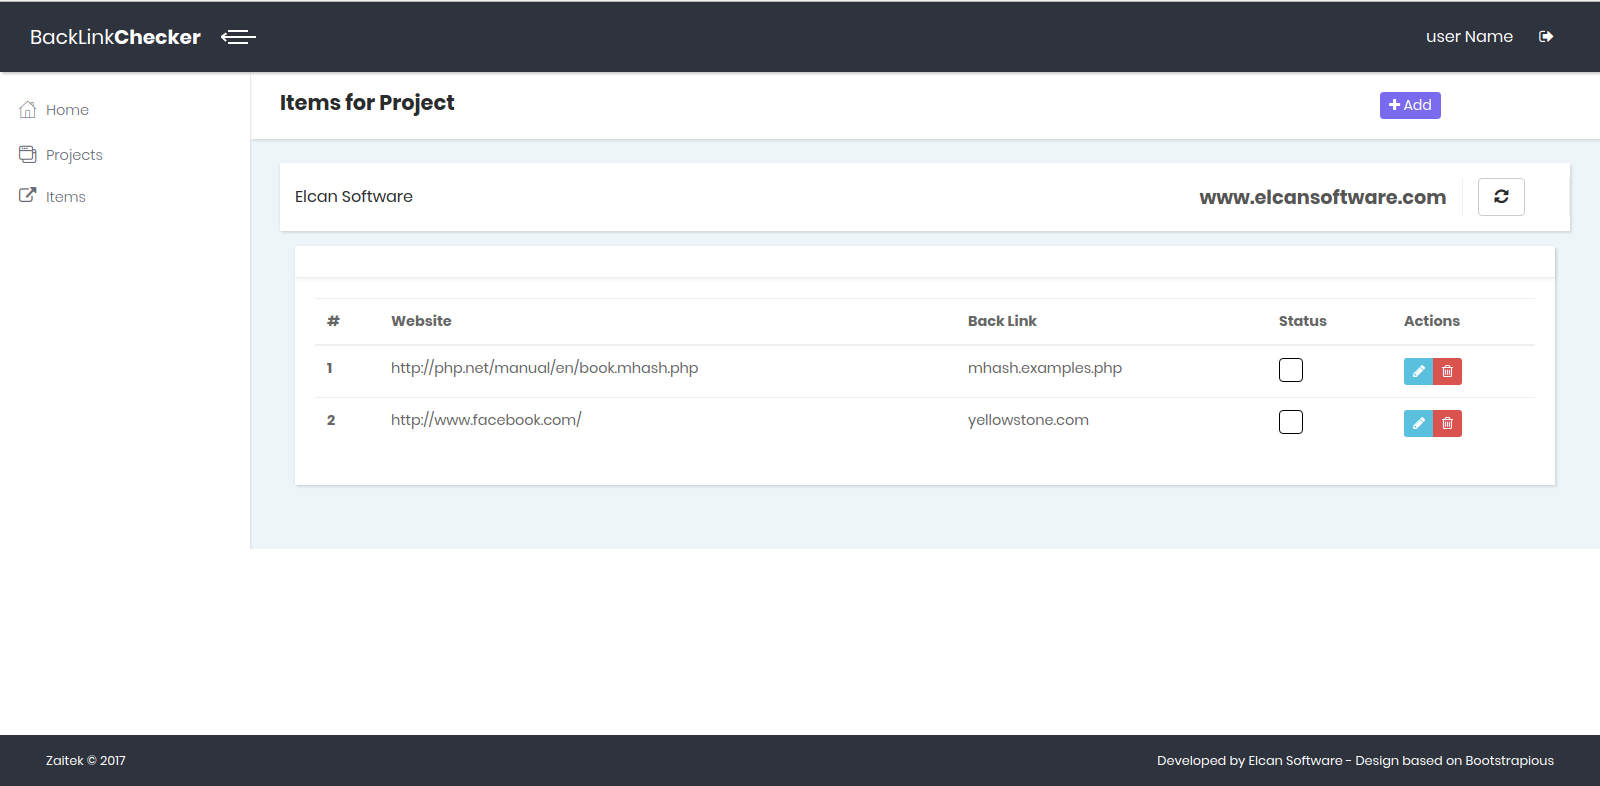
\includegraphics[width=\textwidth]{images/items_for_project}
\end{figure}
The buttons shown here are explained on the items section, on page \pageref{sec:item}.

The delete option sends everything to the trash bin, where the admin can chose to restore or delete the item permanently, when you click delete, the system will ask you to confirm, as seen below.
\begin{figure}[H]
	\caption{Project Delete Confirmation}
	\label{img:prjdel}
	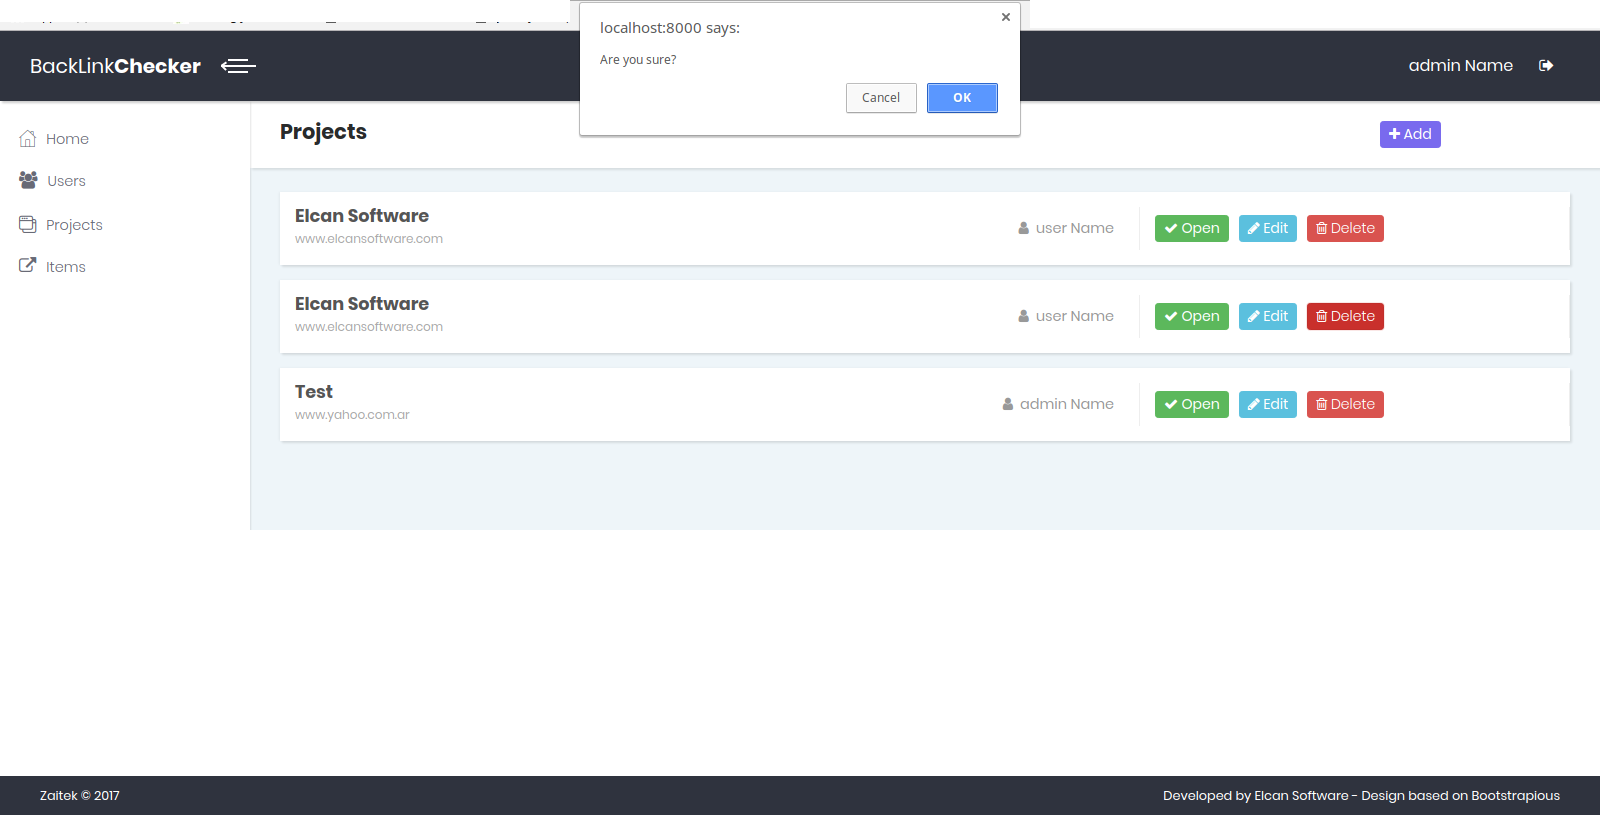
\includegraphics[width=\textwidth]{images/project_delete}
\end{figure}

%%%%%%%%%%%%%%%%%%%%%%%%%%%%%%%%%%%%%
\section{Items}

\label{sec:item}
Items section is accessible to all users, it will show user owned projects and when one is selected, it will display the links to be checked, as shown in the following figure
\begin{figure}[H]
	\caption{Item Main Page}
	\label{img:itmmain}
	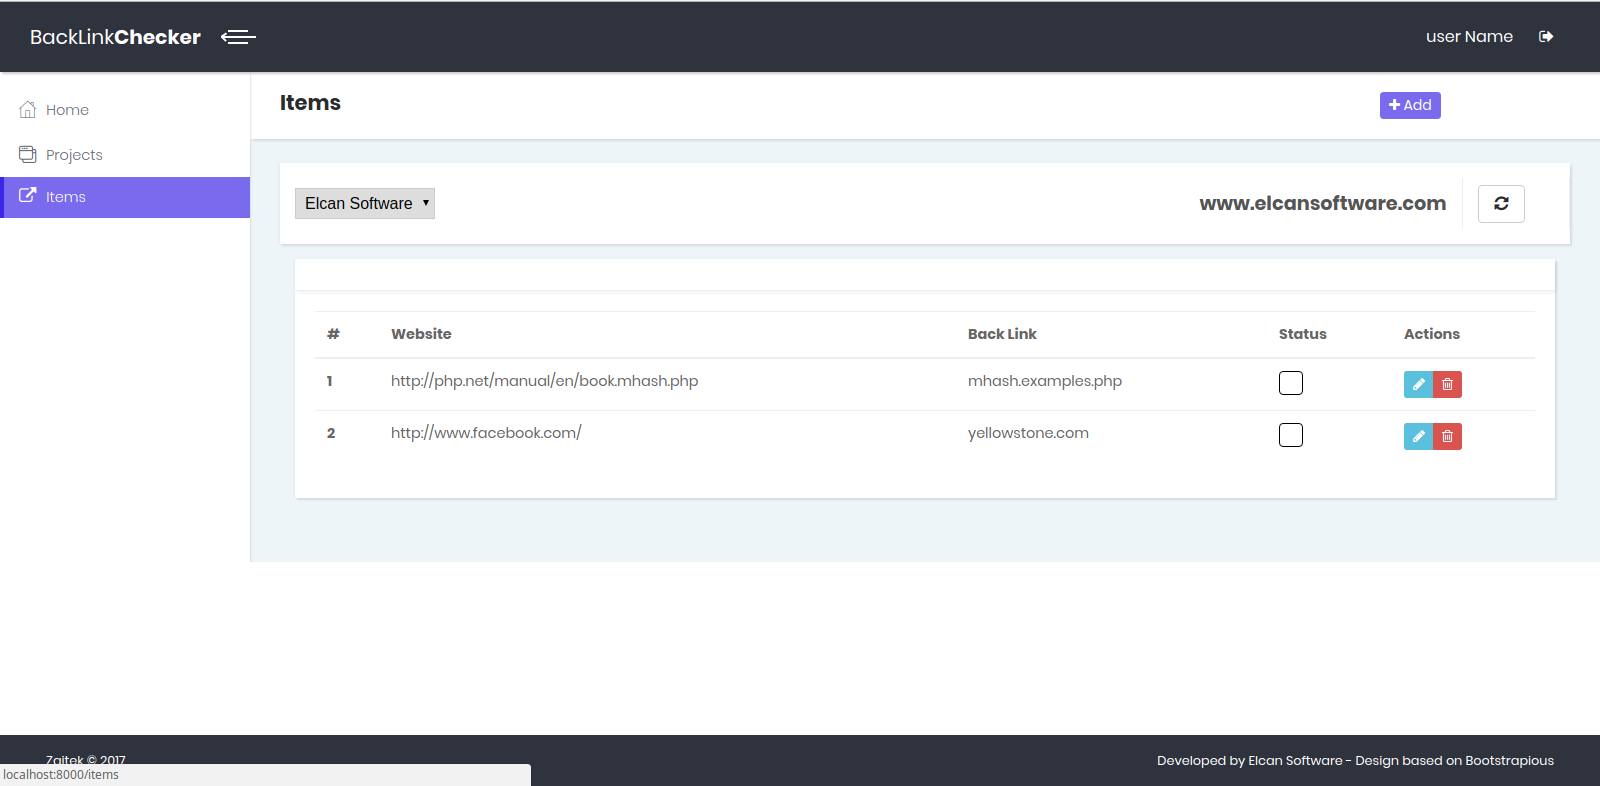
\includegraphics[width=\textwidth]{images/items_main}
\end{figure}

When you click the status check/refresh button the system will show a loading screen, as the following
\begin{figure}[H]
	\caption{Item Status Loading}
	\label{img:itmload}
	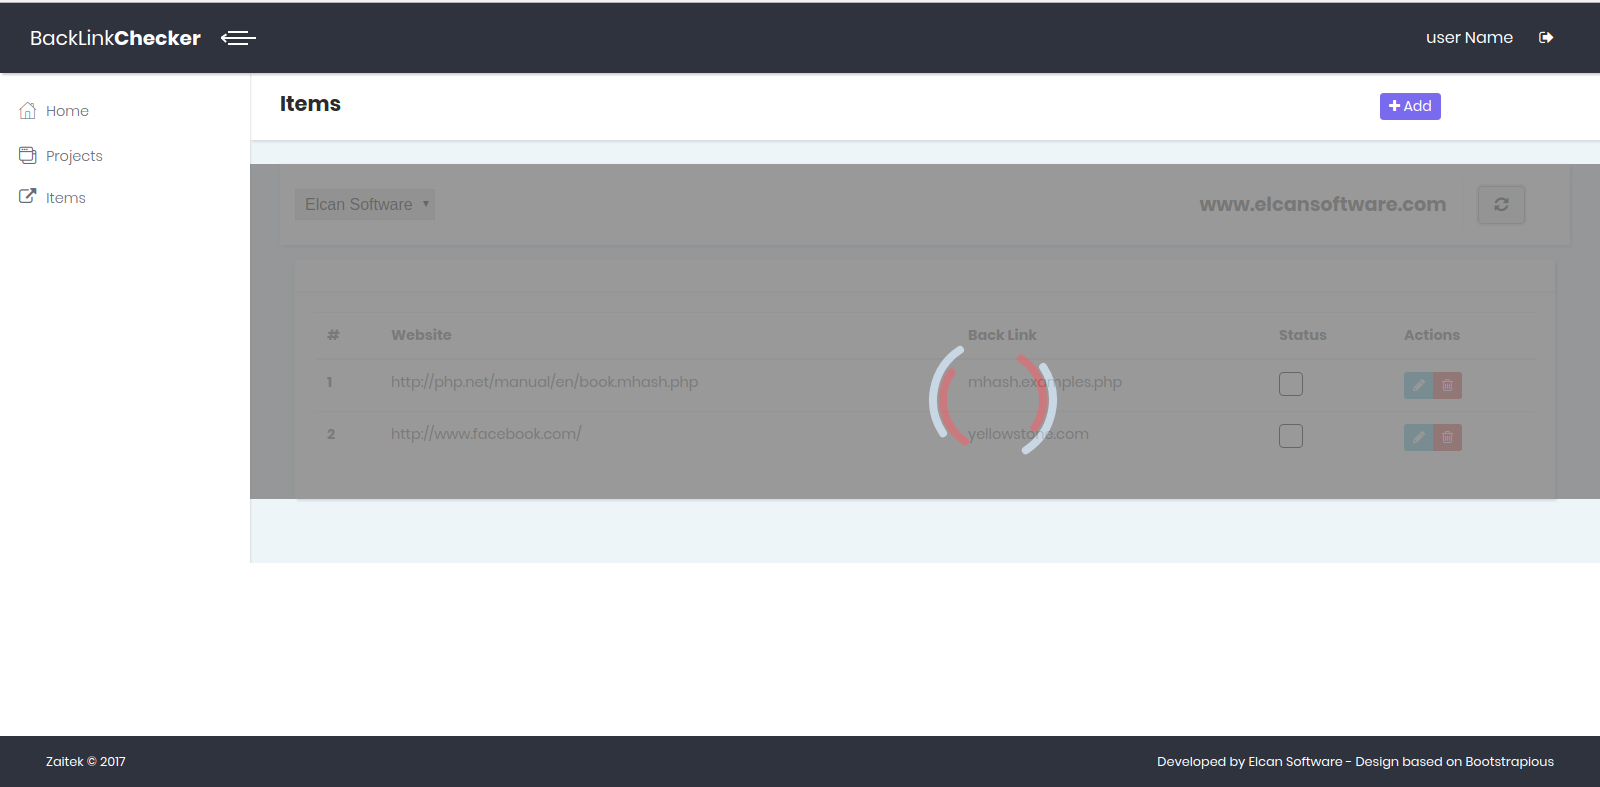
\includegraphics[width=\textwidth]{images/items_loading}
\end{figure}

After some time, when the system has been able to check the data provided, it will show the status icons as listed below:
\begin{figure}[H]
	\caption{Item Status Ready}
	\label{img:itmstat}
	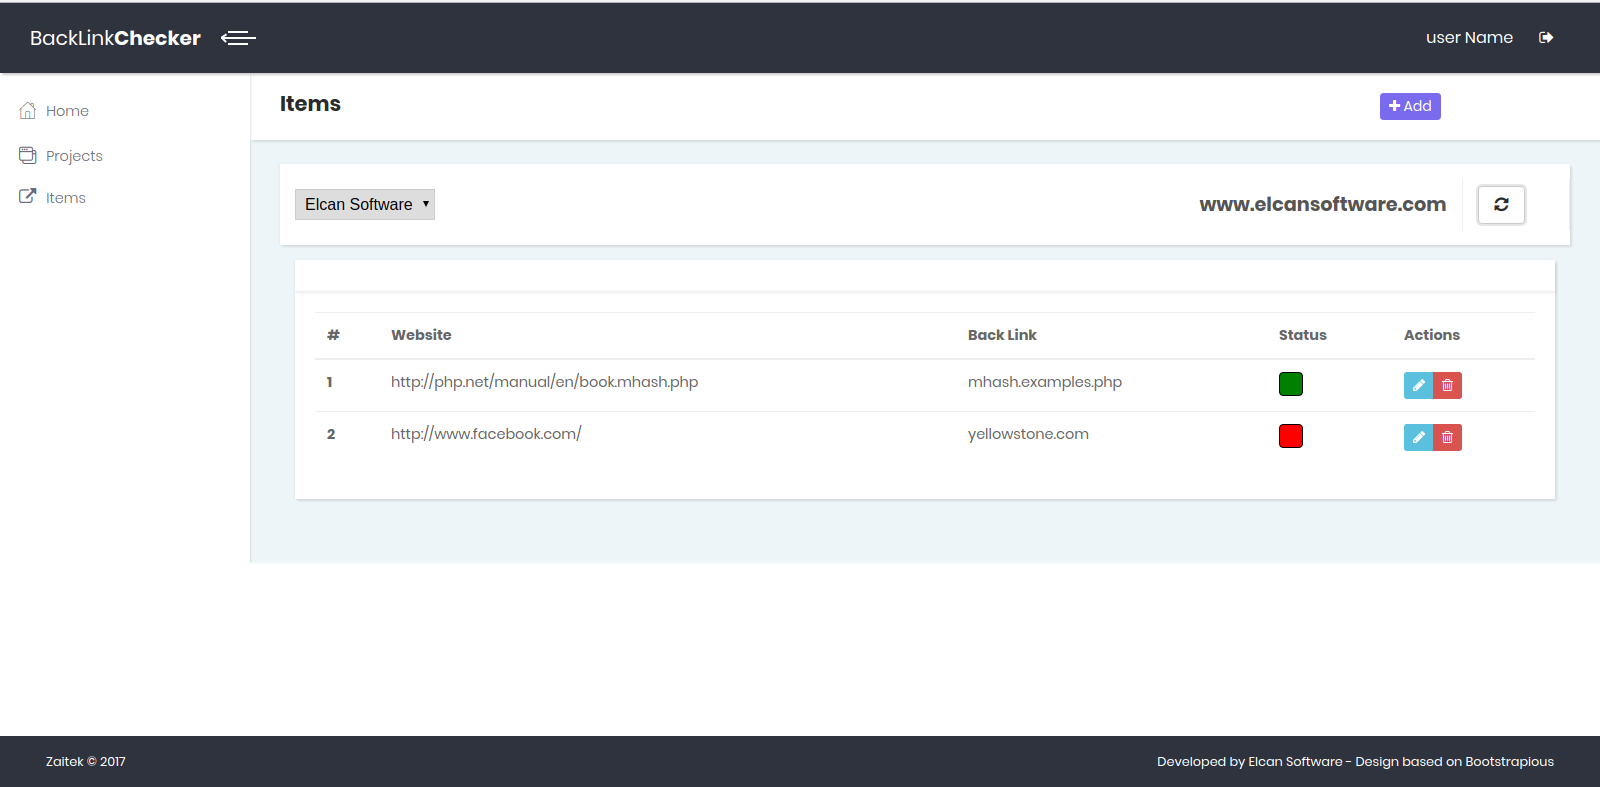
\includegraphics[width=\textwidth]{images/items_status}
\end{figure}

Items can also be edited and deleted as with the project, the interface is shown on figure \ref{img:edititem}.
\begin{figure}[H]
	\caption{Item Edit}
	\label{img:edititem}
	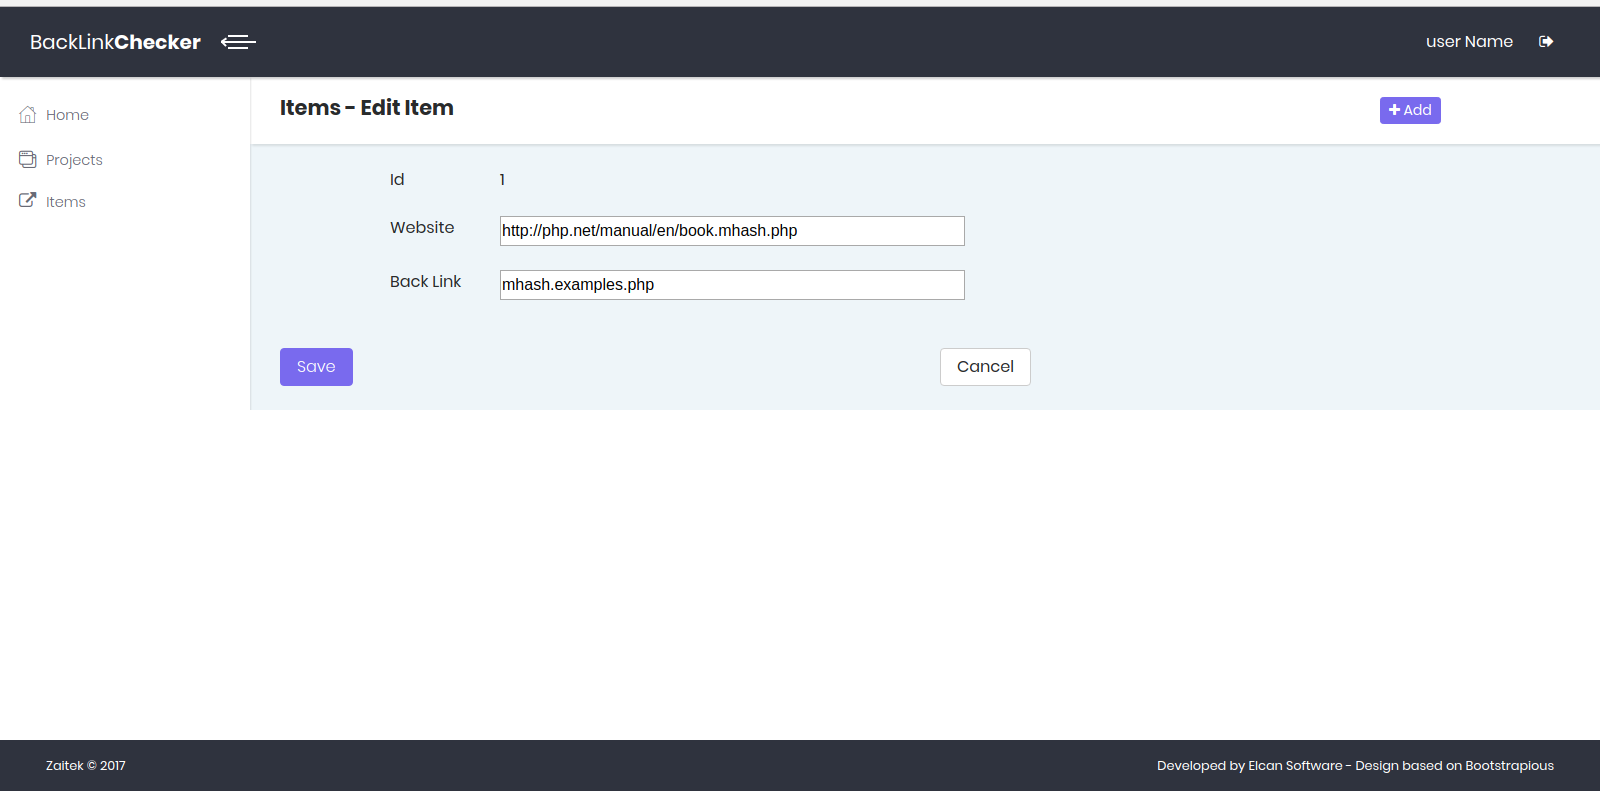
\includegraphics[width=\textwidth]{images/items_edit}
\end{figure}

The item Add form is the same as edit form, but with blank fields so the user can fill them. The only exception is if you click add before selecting the project on the items page, in this case the system will show the following screen:
\begin{figure}[H]
	\caption{Item Add/Create}
	\label{img:itmadd}
	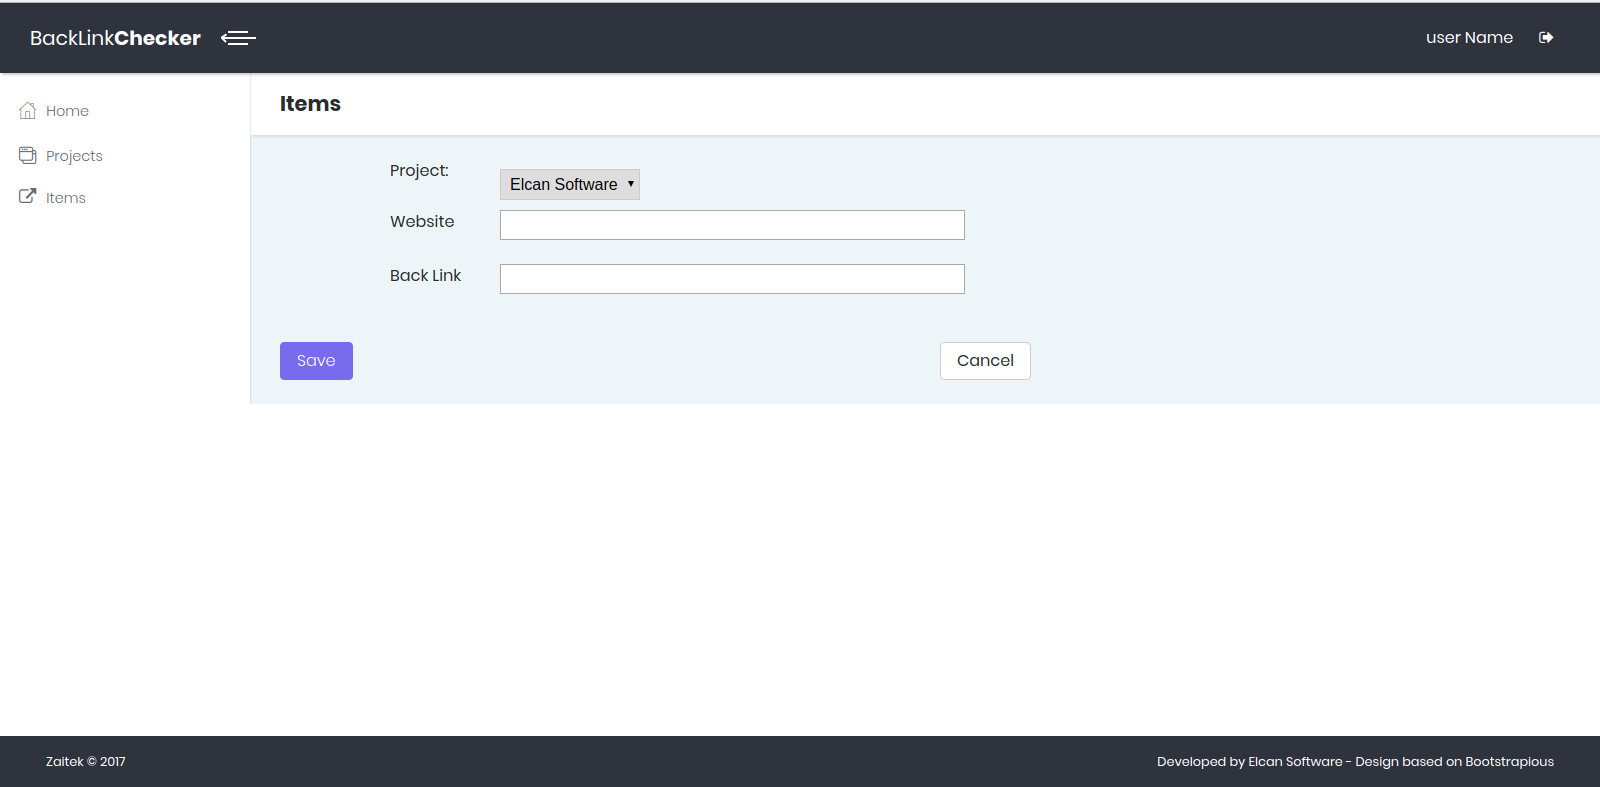
\includegraphics[width=\textwidth]{images/items_add}
\end{figure}
The dropdown on projects must be selected, this will create the item in the proper project.

